\documentclass[12pt,a4paper]{article}
\usepackage{cmap} % Makes the PDF copiable. See http://tex.stackexchange.com/a/64198/25761
\usepackage[T1]{fontenc}
\usepackage[brazil]{babel}
\usepackage[utf8]{inputenc}
\usepackage{amsmath}
\usepackage{amsfonts}
\usepackage{amssymb}
\usepackage{amsthm}
\usepackage[usenames,svgnames,dvipsnames]{xcolor}
\usepackage{hyperref}
\usepackage{multicol}
\usepackage{graphicx}
\usepackage[margin=2cm]{geometry}

\hypersetup{
    colorlinks = true,
    allcolors = {blue}
}

% TODO: Consider using exsheets
% http://linorg.usp.br/CTAN/macros/latex/contrib/exsheets/exsheets_en.pdf
%
% http://ctan.org/tex-archive/macros/latex/contrib/exercise/
% Options: answerdelayed,lastexercise,noanswer
\usepackage[answerdelayed,lastexercise]{exercise}

\addto\captionsbrazil{%
\def\listexercisename{Lista de exerc\'icios}%
\def\ExerciseName{Exerc\'icio}%
\def\AnswerName{Solu\c{c}\~ao do exerc\'icio}%
\def\ExerciseListName{Ex.}%
\def\AnswerListName{Solu\c{c}\~ao}%
\def\ExePartName{Parte}%
\def\ArticleOf{de\ }%
}

\renewcommand{\ExerciseHeaderTitle}{(\ExerciseTitle)\ }
\renewcommand{\ExerciseListHeader}{%\ExerciseHeaderDifficulty%
\textbf{%\ExerciseListName\
\ExerciseHeaderNB.\ %
%\ --- \
\ExerciseHeaderTitle}%
%\ExerciseHeaderOrigin
\ignorespaces}
\renewcommand{\AnswerListHeader}{\textbf{\ExerciseHeaderNB.\ (\AnswerListName)\ }}

\newcommand*\diff{\mathop{}\!\mathrm{d}}
\newcommand*\sen{\operatorname{sen}}

\renewcommand{\theenumi}{\alph{enumi}}
\renewcommand\labelenumi{(\theenumi) }

\newcommand*\tipo{Prova III}
\newcommand*\turma{CIV241-02U}
\newcommand*\disciplina{CDI2002}
\newcommand*\eu{Helder G. G. de Lima}
\newcommand*\data{05/12/2024}

\author{\eu}
\title{\tipo - \disciplina}
\date{\data}

\begin{document}
\thispagestyle{empty}
\newgeometry{margin=2cm,bottom=0.5cm}
\begin{center}

\includegraphics[width=9.0cm]{marca} \\
\textbf{\tipo\ (\disciplina / \turma)} \\
Prof. \eu\footnote{
Este é um material de acesso livre distribuído sob os termos da licença \href{https://creativecommons.org/licenses/by-sa/4.0/deed.pt_BR}{Creative Commons BY-SA 4.0}}
\end{center}

\noindent Nome do(a) aluno(a): \underline{\hspace{9,7cm}} Data: \underline{\data}

\begin{center}\fbox{
\begin{minipage}{14cm}

{\footnotesize
\begin{itemize}
\renewcommand{\theenumi}{\Roman{enumi}}
\item Identifique-se em todas as folhas.
\item Não é permitido o uso de calculadora.
\item Mantenha o celular e os demais equipamentos eletrônicos desligados durante a prova.
\item Justifique cada resposta com cálculos ou argumentos baseados na teoria estudada.
\item Resolva $4$ das $5$ questões (deixe claro que questão não deverá ser corrigida).
\end{itemize}
}

\end{minipage}
}
\end{center}

\begin{ExerciseList}
\Exercise[title={2,5}] Seja $f(x, y) = \frac{x y}{x^2 + y^2}$. Mostre que $\displaystyle\lim_{\begin{smallmatrix} x \to 0 & \\ y \to 0 \end{smallmatrix}} f(x, y)$ não existe e que $\displaystyle\lim_{\begin{smallmatrix} x \to 0 & \\ y \to 0 \end{smallmatrix}} y \cdot f(x, y)$ existe.
\Answer Considerando o caminho $y=x$, o limite de $f$ é $\frac{1}{2}$ e considerando o caminho $y=-x$, o limite de $f$ é $-\frac{1}{2}$.
Por outro lado,
\[
\lim_{\begin{smallmatrix} x \to 0 & \\ y \to 0 \end{smallmatrix}} y \cdot f(x, y)
= \lim_{\begin{smallmatrix} x \to 0 & \\ y \to 0 \end{smallmatrix}} \frac{x y^2}{x^2 + y^2}
= \lim_{\begin{smallmatrix} x \to 0 & \\ y \to 0 \end{smallmatrix}} x \cdot \frac{y^2}{x^2 + y^2}.
\]
Como $\left|\frac{y^2}{x^2 + y^2}\right| \leq 1$ e $\lim_{\begin{smallmatrix} x \to 0 & \\ y \to 0 \end{smallmatrix}} x = 0$, o limite do produto também é zero.

\Exercise[title={2,5}] Classifique, se possível, os pontos críticos da função $f(x, y) = (y^2 + 1) x e^x$.
\Answer Os pontos críticos de $f(x, y)$ ocorrem quando as derivadas parciais de $f$ em relação a $x$ e $y$ são iguais a zero. Temos:
\[
\frac{\partial f}{\partial x}(x, y)
= \frac{\partial}{\partial x} \left[(y^2 + 1)x e^x \right]
= (y^2 + 1) \frac{\partial}{\partial x} \left[x e^x \right]
= (y^2 + 1)\left(e^x + x e^x\right)
= (y^2 + 1)e^x(x + 1).
\]
e
\[
\frac{\partial f}{\partial y}(x, y)
= \frac{\partial}{\partial y} \left[(y^2 + 1)x e^x \right]
= \frac{\partial}{\partial y} \left[(y^2 + 1)\right] \cdot x e^x
= 2y x e^x.
\]

Para encontrar os pontos críticos, resolvemos o sistema:
\[
\begin{cases}
    (y^2 + 1)e^x(x + 1) &= 0,\\
    2y x e^x & = 0.
\end{cases}
\]

Como $y^2 + 1 > 0$ e $e^x > 0$, a primeira equação implica $x + 1 = 0$, isto é, $x = -1$. Logo, segue da segunda equação que $y = 0$. Assim, o único ponto crítico de $f$ é $(-1, 0)$. Para classificá-lo, usaremos o critério da segunda derivada. Temos:

\begin{itemize}
\item \(\frac{\partial^2 f}{\partial^2 x}(x, y)
= \frac{\partial}{\partial x} \big[(y^2 + 1)(e^x + x e^x)\big]
= (y^2 + 1)(x + 2)e^x\)
\item \(\frac{\partial^2 f}{\partial y\partial x}(x, y)
= \frac{\partial^2 f}{\partial x\partial y}(x, y)
= 2y(x + 1)e^x
\)
\item \(
\frac{\partial^2 f}{\partial^2 y}(x, y)
= \frac{\partial}{\partial y} \big[2y x e^x\big]
= 2x e^x.
\)
\end{itemize}
Então, o determinante da matriz Hessiana é:
\[
H
= H(-1, 0)
= \begin{vmatrix}
    \frac{\partial^2 f}{\partial^2 x}(-1, 0) & \frac{\partial^2 f}{\partial x\partial y}(-1, 0) \\
    \frac{\partial^2 f}{\partial y\partial x}(-1, 0) & \frac{\partial^2 f}{\partial^2 y}(-1, 0)
\end{vmatrix}
= \begin{vmatrix}
    e^{-1} & 0 \\
    0 & -2 e^{-1}
\end{vmatrix}
= -2e^{-2}.
\]

Como $H = -2e^{-2} < 0$, o ponto crítico $(-1, 0)$ é um \textbf{ponto de sela}.

\Exercise[title={2,5}] Use conceitos do cálculo diferencial para estimar $\frac{\ln(1,38)}{\cos(0,64)}$.
\Answer Considerando $z = f(x, y) = \frac{\ln(x)}{\cos(y)}$, o objetivo é obter o valor aproximado de $f(1,38, 0,64)$. Como $(1,38, 0,64)$ está próximo do ponto $(1, 0)$, pode-se obter a aproximação linear de $f$ em $(1, 0)$, e usá-la para estimar o valor procurado, já que para pontos $(x, y)$ em uma vizinhança de $(1, 0)$, tem-se:
\[
  f(x, y) \approx f(1, 0) + \frac{\partial f}{\partial x}(1, 0)(x - 1) + \frac{\partial f}{\partial y}(1, 0)(y - 0).
\]
Mas $f(1, 0) = \frac{\ln(1)}{\cos(0)} = \frac{0}{1} = 0$ e
\[
  \frac{\partial f}{\partial x}(x, y)
  = \frac{1}{x\cos(y)}
  \quad\text{ e }\quad
  \frac{\partial f}{\partial y}(x, y)
  = \frac{\ln(x)\sen(y)}{\cos^2(y)}.
\]
Em particular, $\frac{\partial f}{\partial x}(1, 0) = \frac{1}{1\cdot \cos(0)} = 1$ e $\frac{\partial f}{\partial x}(x, y) =\frac{\ln(1)\sen(0)}{\cos^2(0)} = 0$. Portanto,
\begin{align*}
  \frac{\ln(1,38)}{\cos(0,64)}
  & = f(1,38, 0,64)
    \approx 0 + 1 \cdot (1,38 - 1) + 0\cdot (0,64 - 0)
    = 0,38.
\end{align*}
\textit{Observação}: Apenas para fins de comparação, o valor exato, arredondado com seis dígitos corretos após a vírgula é $0,401552$.

\Exercise[title={2,5}]
Seja \( D \) a região entre as circunferências \( x^2 + y^2 = \pi^2 \) e \( x^2 + y^2 = 4\pi^2 \). Utilize coordenadas polares para calcular a integral dupla
\[
\iint_{D} \cos(\sqrt{x^2 + y^2}) \diff{A}.
\]

\Answer
A integral dupla sobre \( D \) é dada por
\begin{align*}
  \iint_{D} \cos(\sqrt{x^2 + y^2}) \diff{A}
  & = \int_0^{2\pi} \int_{\pi}^{2\pi} \cos(r) \cdot |r| \diff{r} \diff{\theta}
    = \int_{\pi}^{2\pi} \int_0^{2\pi} r \cos(r) \diff{\theta} \diff{r} \\
  & = \int_{\pi}^{2\pi} \left[ r \cos(r) \cdot \theta \right]_{\theta=0}^{2\pi} \diff{r}
    = 2\pi \int_{\pi}^{2\pi} r \cos(r) \diff{r}.
\end{align*}

Integrando por partes com \( u = r \), \( \diff{u} = \diff{r} \), \( \diff{v} = \cos(r) \diff{r} \) e \( v = \sen(r) \), tem-se:
\begin{align*}
  \iint_{D} \cos(\sqrt{x^2 + y^2}) \diff{A}
  & = 2\pi \left[ \left( r \sen(r) \right) \bigg|_{\pi}^{2\pi} - \int_{\pi}^{2\pi} \sen(r) \diff{r} \right] \\
  & = 2\pi \left[ \left( 2\pi \sen(2\pi) - \pi \sen(\pi) \right) - \left( -\cos(r) \bigg|_{\pi}^{2\pi} \right) \right] \\
  & = 2\pi \left[ 0 - 0 + \left( \cos(2\pi) - \cos(\pi) \right) \right]
    = 2\pi \left[ 1 + 1 \right]
    = 4\pi.
\end{align*}

\Exercise[title={2,5}] Calcule as integrais iteradas $\int_{0}^{1}\int_{x}^{1}\int_{-1}^{e} 2e^{y^2} \diff{z}\diff{y}\diff{x}$, mudando a ordem de integração, se necessário.
\Answer
Seja $S	= \{(x, y, z) \in \mathbb{R}^3 \mid 0 \leq x \leq 1, \ x \leq y \leq 1 \text{ e } -1 \leq z \leq 1 \}$. Então:
\[
\int_{0}^{1}\int_{x}^{1}\int_{-1}^{e} 2e^{y^2} \diff{z}\diff{y}\diff{x}
 = \iiint_{S} 2e^{y^2} \diff{V}.
\]

\begin{center}
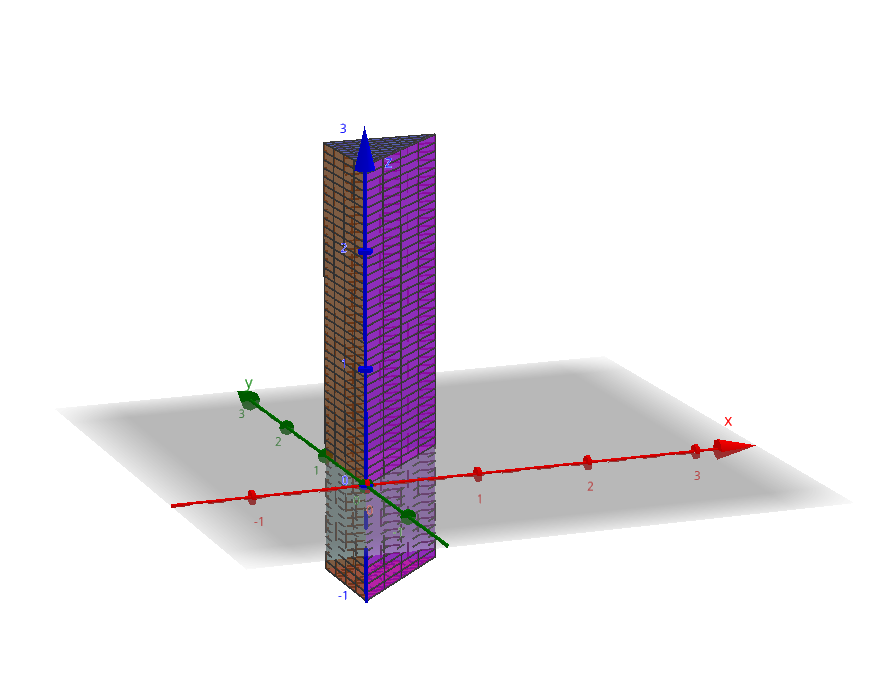
\includegraphics[width=0.5\textwidth]{img/integral-tripla-prisma.png}
\end{center}

Reescrevendo $S = \{(x, y, z) \in \mathbb{R}^3 \mid -1 \leq z \leq e \text{ e } 0 \leq y \leq 1 \text{ e } 0 \leq x \leq y \}$, obtém-se:
\begin{align*}
\iiint_{S} 2e^{y^2} \diff{V}
& = \int_{-1}^{e} \int_{0}^{1}\int_{0}^{y} 2e^{y^2} \diff{x}\diff{y}\diff{z}
  = \int_{-1}^{e} \int_{0}^{1} \left.\left(2xe^{y^2}\right)\right|_{x=0}^{x=y}\diff{y}\diff{z} \\
& = \int_{-1}^{e} \int_{0}^{1} 2ye^{y^2} \diff{y} \diff{z}
  = \int_{-1}^{e} \left.\left(e^{y^2}\right)\right|_{y=0}^{y=1} \diff{z}
  = \int_{-1}^{e} e - 1 \diff{z} \\
& = (e - 1)(z)\big|_{z=-1}^{z=e}
  = (e - 1)(e + 1)
  = e^2 - 1.
\end{align*}
\end{ExerciseList}

\vfill
\begin{center}
BOA PROVA E BOAS FÉRIAS!
\end{center}

\newpage
\restoregeometry
\section*{Respostas}
\shipoutAnswer
\end{document}
